\documentclass[bachelor,euler,twoside,openright]{ustcthesis}
% 默认twoside 双面打印
% 将master修改为bachelor, doctor or master
% 要使用adobe字体,添加adobefonts选项
% 要使用Mac系统的字体,添加macfonts选项
% 使用euler数学字体,如不愿使用,去掉euler
% 使用外文写作,请添加notchinese

% 设置图形文件的搜索路径
\graphicspath{{figures/}}

%仅用于本示例文档中显示特殊字符串
\usepackage{xltxtra}

%%%%%%%%%%%%%%%%%%%%%%%%%%%%%%
%% 封面部分
%%%%%%%%%%%%%%%%%%%%%%%%%%%%%%

  % 中文封面内容
  \title{这里是标题\\标题只能有三行\\不能多}%一般情况下扉页和封皮、书脊共用一个标题文本,可以不用定义\spinetitle(仅硕博有用), \covertitle(本硕博均有用)和\encovertitle(仅本科有用)。特殊情况见下。
  \spinetitle{\small{中国科学技术大学本硕博毕业论文模板示例文档\raisebox{-3pt}{(Beta)}}}
  %特殊情况1:本例中\title命令里含有换行控制字符,这会导致制作书脊的时候出现错误,例如如果你注释掉\spinetitle{...}这一行就会报错。这时需要定义一个不含换行等命令的\spinetitle,这并不表示\spinetitle里不能有任何命令——只能使用有限的命令。
  %特殊情况2:本例中标题过长,所以需要缩小书脊标题的字号。
  %特殊情况3:本例中中英文混排,由于tex竖排的原理限制,中英文基线不重合,所以需要人工调整英文的基线。具体调整量根据不同字体有所不同。
  \covertitle{中国科学技术大学本硕博毕业\\论文模板示例文档(Beta)}
  %\covertitle{中文题目第一行\\中文题目第二行}
  %不要在此调整封皮字体大小! Do not set Cover Page font size here!
  %特殊情况4:本例中\title中含有多个换行,导致标题超过了两行。根据制本厂规定,封皮标题不能超过两行。因此需要定义封皮使用的标题\covertitle. 如果你注释掉这一行,就会发现封皮不符合规定。
  \encovertitle{USTC Thesis Template for Bachelor, Master and Doctor User's Guide(Beta)}
  %\encovertitle{English Title Line 1\\English Title Line 2\\English Title Line 3}
  %不要在此调整封皮字体大小! Do not set Cover Page font size here!
  %特殊情况5:仅本科生有用。本科封皮中有英文标题,不超过三行。与上类似。

  \author{wy\ wfd\ zsq}
  \depart{少年班学院}%系别,硕博请用系代号,本科请用全称如
  %\depart{数理化和信息工程系}
  %\major{人文管理和生物专业专业}%专业,硕博请用全称,本科不需要
  \advisor{黄章进\ 副教授}
  %\coadvisor{冯晨珠\ 教授}%第二导师,没有请注释掉
  %\studentid{PB00000000}%For bachelor only
  \submitdate{二〇一七年五月}

  % 英文封面内容
  %\entitle{USTC Thesis Template for Bachelor, Master and Doctor\\User's Guide(Beta)}
  %\enauthor{Qiansun Zhao}
  %\enmajor{Whatever}
  %\enadvisor{Prof. Wuzheng Zhou}
  %\encoadvisor{Prof. Chenzhu Feng}%另外一个导师
  %\ensubmitdate{Thimber, 2099}
  
%%%%%%%%%%%%%%%%%%%%%%%%%%%%%%%%%%%%%%%%%%%%%%%%%%%%%%%%%%%%%%%%%%%%%
% If you use another language instead of chinese or english, then you
% should define some strings and provide information in your language.
%%%%%%%%%%%%%%%%%%%%%%%%%%%%%%%%%%%%%%%%%%%%%%%%%%%%%%%%%%%%%%%%%%%%%
%  \otherustcstr{zhong guo ke xue ji shu da xue}%A translation of `University of Science and Technology of China' in your language
%  \otherthesisstr{shuo shi xue wei lun wen}%A translation of `A dissertation for doctor(master/bachelor)'s degree' in your language
%  \otherauthorstr{xing ming}%A translation of `Author' in your language
%  \otherdepartmentstr{yuan xi}%A translation of `Department' in your language
%  \otherstudentidstr{xue hao}%A translation of `Student ID' in your language
%  \othersupervisorstr{dao shi}%A translation of `Supervisor' in your language
%  \otherfinishedtimestr{ri qi}%A translation of `Finished Time' in your language
%  \otherspecialitystr{zhuan ye}%A translation of `Speciality' in your language
%  \othertitle{zhong guo ke xue ji shu da xue tong yong xue wen lun wen shi li wen dang}
%  \otherauthor{zhao qian sun}
%  \otheradvisor{zhou wu zheng}
%  \othercoadvisor{feng chen zhu}
%  \othersubmitdate{hou nian ma yue}
%  \othermajor{mou zhuan ye}
%  \otherdepart{mou xi}

\begin{document}

  % 封面
  \maketitle

%特别注意,以下述顺序为准,在对应部分添加文档部件,切勿颠倒顺序:
%本科论文的文档部件顺序是:
%    frontmatter:致谢、目录、中文摘要、英文摘要、
%    mainmatter: 正文章节
%    backmatter: 参考文献或资料注释、附录
%硕博论文的文档部件顺序是:
%    frontmatter:中文摘要、英文摘要、目录、符号说明
%    mainmatter: 正文章节
%    backmatter: 参考文献、附录、致谢、发表论文
%%%%%%%%%%%%%%%%%%%%%%%%%%%%%%
%% 前言部分
%%%%%%%%%%%%%%%%%%%%%%%%%%%%%%
\frontmatter
\makeatletter
\ifustc@bachelor
	%%%%%%%%%%%%%%%%%
	%本科论文修改这里
	%%%%%%%%%%%%%%%%%
	% 致谢
	
\begin{thanks}

感谢原本科模板的作者XPS、硕博模板的作者刘青松以及它们的维护者的辛勤工作!

感谢大家对本模板更新工作的支持!

本模板以及本示例文档还存在许多不足之处,欢迎大家测试并及时提供反馈。

\begin{flushright}
ywg@USTC
\end{flushright}


在中国科技大学完成本科和硕博连读学业的九年里,我所从事的学习和研究工作,都是在导师以及系里其他老师和同学的指导和帮助下进行的。在完成论文之际,请容许我对他们表达诚挚的谢意。

首先感谢导师XXX教授和XXX副教授多年的指导和教诲,是他们把我带到了计算机视觉的研究领域。X老师严谨的研究态度及忘我的工作精神,X老师认真细致的治学态度及宽广的胸怀,都将使我受益终身。

感谢班主任XXX老师和XX老师多年的关怀。感谢XXX、XX、XX等老师,他们本科及研究生阶段的指导给我研究生阶段的研究工作打下了基础。

感谢XX、XXX、XXX、XX、XXX、XXX、XXX、XX等师兄师姐们的指点和照顾;感谢XXX、XX、XXX等几位同班同学,与你们的讨论使我受益良多;感谢XXX、XX、XXX、XX、XXX等师弟师妹,我们在XXX实验室共同学习共同生活,一起走过了这段愉快而难忘的岁月。

感谢科大,感谢一路走过来的兄弟姐妹们,在最宝贵年华里,是你们伴随着我的成长。

最后,感谢我家人一贯的鼓励和支持,你们是我追求学业的坚强后盾。

\vskip 18pt

\begin{flushright}

~~~~赵钱孙~~~~

\today

\end{flushright}

\end{thanks}

	
	%目录部分
	%目录
	\tableofcontents
	%默认表格、插图、算法索引名称分别为“表格索引”、“插图索引”和“算法索引”
	%如果需要自行修改lot,lof,loa的名称,请定义
	%\ustclotname{...}
	%\ustclofname{...}
	%\ustcloaname{...}

	% 表格索引
	\ustclot
	% 插图索引
	\ustclof
	%算法索引 
	%如果需要使用算法环境并列出算法索引,请加入补充宏包。
	\ustcloa
	
	% 摘要
	\begin{cnabstract}
增强现实是一种在现实场景中无缝地融入虚拟物体或信息的技术,能够比传统的文字,图像和视频等方式更高效、直观地呈现信息,有着非常广泛的应用。同时定位与地图构建作为增强现实的关键基础技术,可以用来在未知环境中定位自身方位并同时构建环境三维地图,从而保证叠加的虚拟物体与现实场景在几何上的一致性。文中首先简述基于视觉的同时定位与地图构建的基本原理并简单比较不同单目同时定位与地图构建技术的优劣,然后详细介绍了基于关键帧的单目相机实时重建的PTAM算法,而后探究了PTAM算法的改进ORB-SLAM算法,并提出了几点在家居设计和增强现实中的应用构想。最后讨论了动态环境下SLAM算法的改进,最后讨论近年来SLAM的发展趋势,并做总结和展望。

\keywords{同时定位与地图构建\enskip 增强现实\enskip 多视图几何\enskip 动态SLAM技术\enskip PTAM算法\enskip ORB-SLAM算法}
\end{cnabstract}

%\begin{enabstract}
%This is USTC thesis template for bachelor, master and doctor user's guide. The template is created by ywg@USTC and a derivative of USTC Bachelor and Master-PhD templates. Besides that
%the usage of the template, a brief
%guideline for writing thesis is also provided.
%
%\enkeywords{University of Science and Technology of China (USTC), Thesis, Universal \LaTeX{} Template, Bachelor, Master, PhD}
%\end{enabstract}
%此文件中含有中英文摘要
\else
	%%%%%%%%%%%%%%%%%
	%硕博论文修改这里
	%%%%%%%%%%%%%%%%%
	% 摘要
	\begin{cnabstract}
增强现实是一种在现实场景中无缝地融入虚拟物体或信息的技术,能够比传统的文字,图像和视频等方式更高效、直观地呈现信息,有着非常广泛的应用。同时定位与地图构建作为增强现实的关键基础技术,可以用来在未知环境中定位自身方位并同时构建环境三维地图,从而保证叠加的虚拟物体与现实场景在几何上的一致性。文中首先简述基于视觉的同时定位与地图构建的基本原理并简单比较不同单目同时定位与地图构建技术的优劣,然后详细介绍了基于关键帧的单目相机实时重建的PTAM算法,而后探究了PTAM算法的改进ORB-SLAM算法,并提出了几点在家居设计和增强现实中的应用构想。最后讨论了动态环境下SLAM算法的改进,最后讨论近年来SLAM的发展趋势,并做总结和展望。

\keywords{同时定位与地图构建\enskip 增强现实\enskip 多视图几何\enskip 动态SLAM技术\enskip PTAM算法\enskip ORB-SLAM算法}
\end{cnabstract}

%\begin{enabstract}
%This is USTC thesis template for bachelor, master and doctor user's guide. The template is created by ywg@USTC and a derivative of USTC Bachelor and Master-PhD templates. Besides that
%the usage of the template, a brief
%guideline for writing thesis is also provided.
%
%\enkeywords{University of Science and Technology of China (USTC), Thesis, Universal \LaTeX{} Template, Bachelor, Master, PhD}
%\end{enabstract}
%此文件中含有中英文摘要
	% 目录
	\tableofcontents
	%默认表格、插图、算法索引名称分别为“表格索引”、“插图索引”和“算法索引”
	%如果需要自行修改lot,lof,loa的名称,请定义
	%\ustclotname{...}
	%\ustclofname{...}
	%\ustcloaname{...}

	% 表格索引
	\ustclot
	% 插图索引
	\ustclof
	%算法索引 
	%如果需要使用算法环境并列出算法索引,请加入补充宏包。
	\ustcloa
	
	%符号说明,需要加入补充包
	\begin{denotation}

\item[HPC] 高性能计算 (High Performance Computing)
\item[cluster] 集群
\item[Itanium] 安腾
\item[SMP] 对称多处理
\item[API] 应用程序编程接口
\item[PI]	聚酰亚胺
\item[MPI]	聚酰亚胺模型化合物,N-苯基邻苯酰亚胺
\item[PBI]	聚苯并咪唑
\item[MPBI]	聚苯并咪唑模型化合物,N-苯基苯并咪唑
\item[PY]	聚吡咙
\item[PMDA-BDA]	均苯四酸二酐与联苯四胺合成的聚吡咙薄膜
\item[$\Delta G$]  	活化自由能~(Activation Free Energy)
\item [$\chi$] 传输系数~(Transmission Coefficient)
\item[$E$] 能量
\item[$m$] 质量
\item[$c$] 光速
\item[$P$] 概率
\item[$T$] 时间
\item[$v$] 速度
\end{denotation}
%不是必需的,如果不想列出请注释掉
\fi
\makeatother

%%%%%%%%%%%%%%%%%%%%%%%%%%%%%%
%% 正文部分
%%%%%%%%%%%%%%%%%%%%%%%%%%%%%%
\mainmatter

  %
\chapter{绪论}
\label{chap:introduction}

中国科学技术大学论文模板(ustcthesis)是按照中国科学技术大学学士、硕士和博士论文要求制作的\LaTeX 通用论文模板。其前身是中国科学技术大学本科论文模板(作者XPS,最后维护ywg)和中国科学技术大学研究生论文模板(作者Liuqs,主要维护Liuqs、Guolicai)。本模板在上述两模板基础上进行了整合梳理,将模板的基础实现和增强功能进行分离,分别提供最基础的ustcthesis.cls以及增强包ustcxtra.cls。其中,ustcthesis.cls仅提供模板的最基础格式,ustcxtra.cls则包含一些常用的优化设置及更为便捷的自定义命令。

本文是使用上述模板生成的示例文档,目的在于帮助使用者熟悉该模板的使用方法,并且为使用者学位论文的撰写提供基础代码示例。

\section{系统要求}
\subsection{系统要求}
本模板基于\CTeX 的ctexbook文档类进行定制,基于\XeTeX 引擎排版。使用本模板的最基础功能时,除了上述需求外,还需要如下几类宏包(直接引用):
\begin{description}
\item[数学类]{amsmath、amsthm、amsfonts、amssymb、bm}
\item[格式类]{titletoc、titlesec、geometry、caption}
\item[表格类]{multicol、multirow}
\item[其他]{xparse、xeCJK、hyperref、natbib、subfiles}
\end{description}
可能有部分宏包是由上述宏包以及\CTeX 间接引用的,此处不一一列举。

另外,如果需要使用增强的ustcxtra.cls,额外需要如下宏包(直接引用):
\begin{description}
\item[默认载入]{times、algorithm2e、graphicx、psfrag、subfig、enumerate、epsfig、float、paralist、booktabs、footmisc、wasysym、longtable、bbm、indentfirst、ifthen、caption3、array、fancyvrb、xcolor、url}
\item[条件载入]{eulervm(仅在文档类处于增强模式并在文档类选项注明euler时载入)}
\end{description}

\section{下载与安装}
\subsection{模板文件清单}
使用模板之前请确保模板文件没有缺失损坏。文件清单如\autoref{tab:filelist},标注关键的文件需要确保文件以及路径的完整。
\begin{table}[htp]
\centering
\tabcaption{模板主要文件清单}
\label{tab:filelist}
\begin{tabular}{lll}
\toprule
文件名&相对路径&备注\tabularnewline
\midrule
clean.bat			&./			&清理脚本\tabularnewline
clean.sh			&./			&清理脚本\tabularnewline
main.pdf			&./			&示例文件\tabularnewline
main.tex 			&./			&示例TeX文件\tabularnewline
make.bat			&./			&生成脚本\tabularnewline
make.sh				&./			&生成脚本\tabularnewline
ustcbib.bst		&./			&Bib格式文件\tabularnewline
ustcthesis.cls		&./			&(关键)模板\tabularnewline
ustcxtra.cls		&./			&(关键)模板增强\tabularnewline
ustc\_logo\_fig.eps	&./figures	&(关键)科大校徽\tabularnewline
ustc\_logo\_text.eps&./figures	&(关键)科大校名\tabularnewline
\bottomrule
\end{tabular}
\end{table}

\subsection{模板下载与使用}
由于Google公司决定停止Google Code服务,故原Google Code项目网站的模板整体迁移至GitHub网站并继续进行更新维护。本模板及本示例文件可以在GitHub网
站\url{https://github.com/ywgATustcbbs?tab=repositories}下载。备份托管地址为\url{https://gitlab.lug.ustc.edu.cn/ywg/ustcthesis},此托管网站由LUG@USTC提供服务。

请在项目页面选择ustcthesis->新页面中选择Download Zip下载最新模板文件(\autoref{fig:download})。也可以通过git clone的方式获得模板。

\begin{figure}
\centering
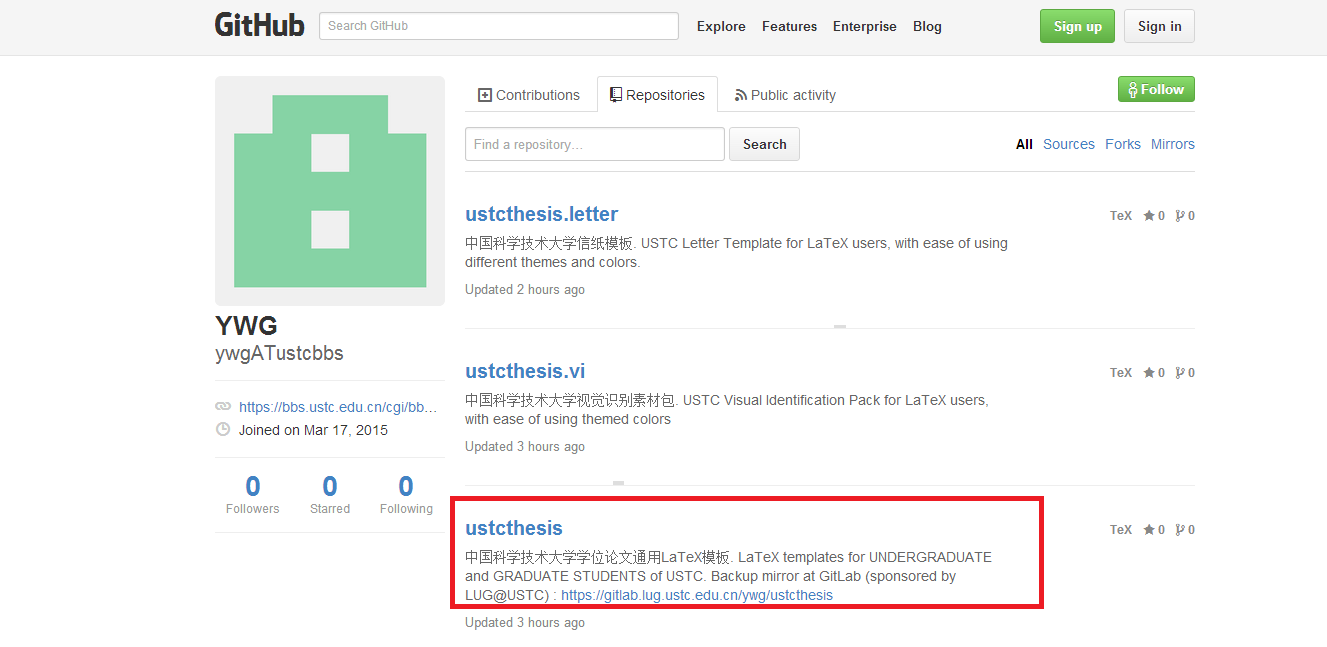
\includegraphics[width=0.48\textwidth]{download}
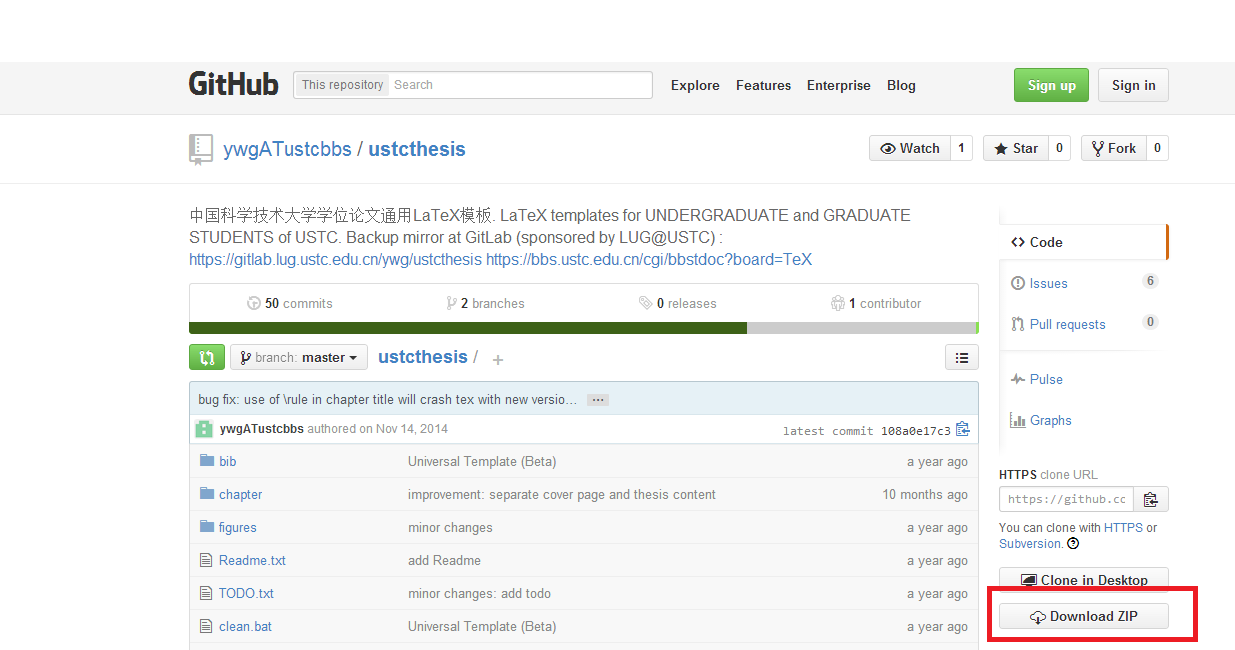
\includegraphics[width=0.48\textwidth]{download1}
\figcaption{在GitHub上进行模板下载}
\label{fig:download}
\end{figure}

\textbf{特别注意1:}本硕博通用论文模板的名称为ustcthesis,其他项目如ustcthesis.vi/ustcthesis.letter/ustcthesis.beamer是用作其他用途的模板,并非本模板所需文件,如对其感兴趣,请进入对应页面了解详情。

\textbf{特别注意2:}此前开发的本科和硕博模板已暂停支持,但仍然可以选择对应的版本(ustcthesis.bachelor和ustcthesis.msphd)进行下载。

模板的安装使用方法有多种,最为简单便捷的方法是直接解压缩下载好的压缩包,修改其中的main.tex文件以及chapter文件夹下的文件,必要时增加所需要的文件。需要注意的是确保所有文件使用UTF-8编码。Windows系统中将其他编码的文件转化为UTF-8的方法是: 用记事本打开这些文件, 然后点击文件—另存为—在最下方选择UTF-8 编码。

\subsection{\texorpdfstring{\LaTeX}{LaTeX}系统的安装和使用}
由于本模板使用了较多的宏包,因此建议使用TeXLive2013及以上版本的\LaTeX 发行版。TeXLive2013可以在Windows、GNU/Linux和大多数Unix系统中运行。对于MacOSX,推荐使用MacTeX-2013。详细信息参考\url{https://www.tug.org/texlive/}。

对于中国科学技术大学的校内用户而言,最方便的获取TeXLive2013的途径是使用LUG@USTC提供的CTAN镜像源(\url{http://mirrors.ustc.edu.cn/CTAN/})。最新的TeXLive位于/CTAN/systems/texlive/目录(\url{http://mirrors.ustc.edu.cn/CTAN/systems/texlive/})内。用户可以选择进入Images文件夹下载完整的光盘并刻录安装,也可以选择进入tlnet文件夹下载运行install-tl.exe进行在线安装。需要注意的是,在线安装的时候可以通过切换安装源为本校镜像源来加快下载安装速度。

对于校外用户,可以通过CTAN.org获得官方的TeXLive。CTAN在全球41个国家和地区分布有115个镜像站点,它们的地址可以在\url{http://www.ctan.org/mirrors/}找到。

\subsection{推荐使用的编辑器}
\LaTeX 的源文件是一个或多个文本文件,这意味着可以使用最为简单的文本编辑器来撰写论文。但是和许多编程语言类似,使用一款带有语法高亮、命令补全等功能的文本编辑器能够大大提升协作效率。

对于不同的编辑器而言,能够实现的功能也不尽相同,加之不同用户拥有不同的使用习惯,简单武断的说某一款编辑器好或者不好有失公允。对于\TeX 写作而言,用户使用的编辑器大致可以分为两类:通用的文本编辑器和专用的GUI编辑器。通用的文本编辑器中公认比较好用的有Vim(Linux)、Emacs(Linux)、Notepad++(Windows)等等\footnote{当然,这些软件可能都有跨平台版本,而且也有其他很多优秀的文本编辑器,不要在意这些细节啦,我并不想挑起编辑器的圣战。:P}。这些编辑器有着强大的功能,但是往往需要在编辑和编译之间来回切换。而专用的GUI编辑器如TeXShop(Mac)、TeXWorks(windows/Linux)和Winedit(Windows、付费软件)等虽然可能在文本编辑上略显笨拙,但是其优点在于编写和生成一体化,简单化。

使用何种编辑器这个问题见仁见智,但是对于一个刚从word转来的新人,从界面简洁、操作简单、功能实用的角度出发,TeXWorks不失为一款优秀的GUI软件,如\autoref{fig:texworks}。

\begin{figure}
\centering
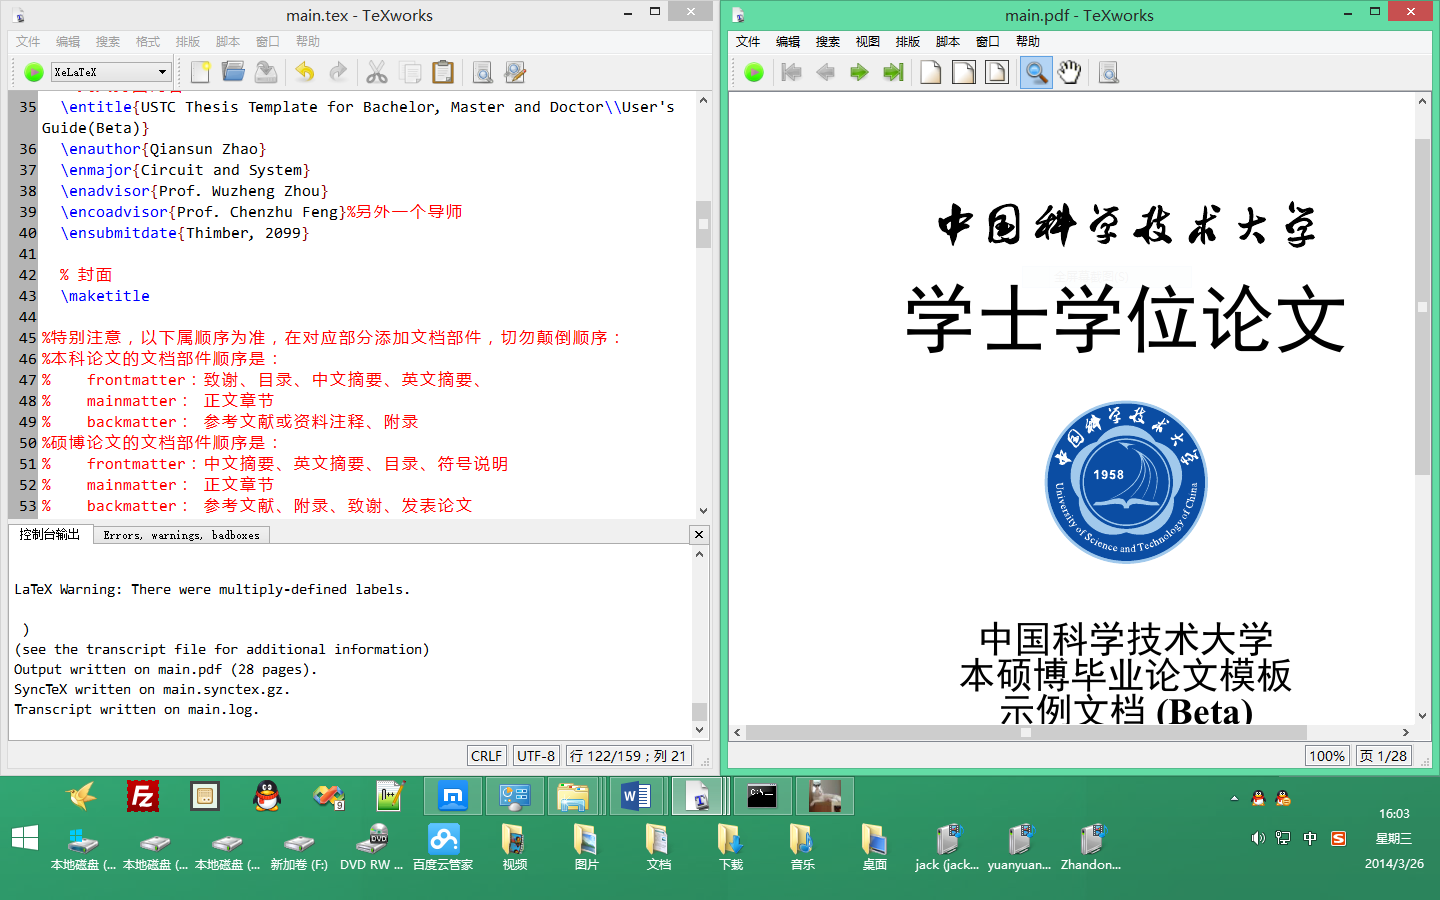
\includegraphics[width=0.9\textwidth]{texworks}
\figcaption{TeXWorks主界面}
\label{fig:texworks}
\end{figure}

Windows系统下TeXWorks的界面拥有左右两个窗口,左边为编辑窗口,右边为预览窗口,当编辑完文档之后,只需点击绿色的开始按钮,就可以立即对文档进行保存并编译,可以选择不同的引擎进行处理。编译过程中的信息会在左侧窗口下方显示。TeXWorks默认UTF-8编码,安装时自动查找TeX安装目录,支持自动缩进、语法高亮、命令补全、正则式查找以及TeX文件和PDF的正反查找(即点击命令跳转到对应pdf文字位置以及点击pdf文字跳转到对应命令,操作是Ctrl+单击)。这些功能对新手来说都是十分友好的。

\section{问题反馈}

如果您在使用过程中有疑问,遇到困难,可以在\href{http://bbs.ustc.edu.cn/cgi/bbsdoc?board=TeX}{瀚海星云\TeX{}讨论区}或者相关的\LaTeX 论坛(如\href{http://bbs.ctex.org}{CTEX 论坛})寻求帮助,但是请注意遵守论坛的各项规定。

如果使用过程中遇到Bug,请提交到\href{http://bbs.ustc.edu.cn/cgi/bbsdoc?board=TeX}{瀚海星云\TeX{}讨论区},或者提交到相应的\href{http://code.google.com/p/ustcthesis/issues/list}{Google UstcThesis Project(http://code.google.com/p/ustcthesis/issues/list)},请注明是什么版本模板的bug。
  
\def \R2{\mathbb{R}^2}
\def \R3{\mathbb{R}^3}
\def \Rn{\mathbb{R}^n}

\def \itW{\mathit{W}}

\def \itK{\mathit{K}}
\def \bfp{\mathbf{p}}

\chapter{基于BA的单目相机实时重建的经典算法(PTAM)介绍}

本章节将重点讨论并实现基于BA的单目相机实时重建经典算法:PTAM。该算法是基于关键帧特征和BA的稀疏重建算法的开山鼻祖,具有重要的意义。

\section{PTAM算法的介绍}
首先我们将简述PTAM\cite{Klein2007}(Parallel Tracking and Mapping)实现单目相机SLAM的原理。单目相机模型(Monocular SLAM)不同于多目相机模型,实时追踪时相机视界中的点不能和其它相机视界中的点进行匹配或者实现三角定位,只能和自己的关键帧匹配,从而加大了3D重建中定位(即深度信息求解)的难度。一般的PTAM算法首次提出利用双线程,将全局BA和相机姿态估计这两个任务分离,从而大幅提高了计算效率,使得单目相机实时追踪特征点,实现三维重建成为可能。

PTAM算法主要思想是将Tracking和Mapping两个过程放在不同的管线(进程)中进行: Tracking 进程专门实现相机位置的估计,Mapping 进程则用于进行关键帧之间的误差消除。

\section{PTAM算法工作的基本流程}
如果记$\itW$为真实世界的坐标系,PTAM算法将维护一个关键帧集合: $Img=\{I_1,I_2,\ldots,I_m\}$,这\(m\)个关键帧分别对应\(m\)个相机坐标系 $\itK_i$,以及一个三维重建的结果。我们用 $E_{\itK_i\itW}$ 表示从世界坐标系到相机坐标系的仿射变换(Affine Transformation)。


\subsection{PTAM管线之一: Tracking}


追踪进程需要解决如下的问题:

当读入了新的关键帧之后,原来算法在重建过程中提取的3维空间中的特征点现在在照片中的坐标是什么?现在的相机姿态应该怎么估计? 

我们假定程序可以从映射进程得到一个关键帧集合 $Img$ 以及3维重建的特征点的坐标集合(相对于世界坐标系)$P=P_\itW=\{\bfp_{1\itW},\ldots,\bfp_{s\itW}\}$,为了统一形式,将第$j$个点坐标记为 $\bfp_{j\itW}= (p_{jx},p_{jy},p_{jz},1)$。

根据已知结论,仿射坐标系变换对应公式为

\begin{equation}
\bfp_{jK_{t+1}}= E_{K_{t+1}\itW} \bfp_{j\itW}
\end{equation}

为了把三维空间中的视界投影到二维空间,算法遵循\cite{Klein2007}中的FOV相机模型,构建一个$\mathbb{R}^3$到 $\mathbb{R}^2$ 的映射为:

\begin{equation}
\label{eq:FOV}
f(x,y,z,1)=(u_0,v_0) + (x/z,y/z) 
\begin{bmatrix}
       f_u  & 0 \\
       0 & f_v  \\
\end{bmatrix} \frac{r'}{r}
\end{equation}
\begin{equation}
r= \sqrt{\frac{x^2+y^2}{z^2}}
\end{equation}

\begin{equation}
r'= \frac{1}{\omega} arctan(2rtan\frac{\omega}{2})
\end{equation}

其中我们假定焦距$f_u,f_v$,主点位置$(u_0,v_0)$和畸变系数$\omega$已知。这时对于实时相机姿态的更新,相当于对于 \autoref{eq:FOV} 求微分,在假定线性运动的情况下更新相机姿态的变换仿射矩阵。若我们设从上一关键帧到下一个关键帧的仿射变换矩阵为$T$,则有以下的关系成立:

\begin{equation}
E_{K_{t+1}\itW}  = T E_{K_{t}\itW} = exp(\mu) E_{K_{t}\itW}
\end{equation}

其中$\mu$为6维向量,代表矩阵 $T$的6个自由度。所以问题转化为: 根据图像中特征点$(u,v)$的变化和在每个特征点三维空间中的预估位置,求解$\mu,T$的取值。


我们假定点$p$为我们需要定位的特征点,则我们首先需要在当前的关键帧图像中找到该点的新投影坐标$(\hat{u},\hat{v})$。为此,我们构造图像的尺度空间,利用 %\citep{}
的FAST-10\cite{Rosten2006}计算角点的方法提取可能的特征点。在假定相机移动很慢的情况下,特征点匹配算法从上一帧的位置开始,在一定的半径阈值内,在对应的视界空间上,依据设计好的评价函数(scoring function)进行搜索。
算法会在搜索过程中得到一个坐标$(\hat{u},\hat{v})$,以及 $\sigma=2^l$ 作为视界空间金字塔中搜索对应的层数。

\begin{figure}[!htbp]
\centering
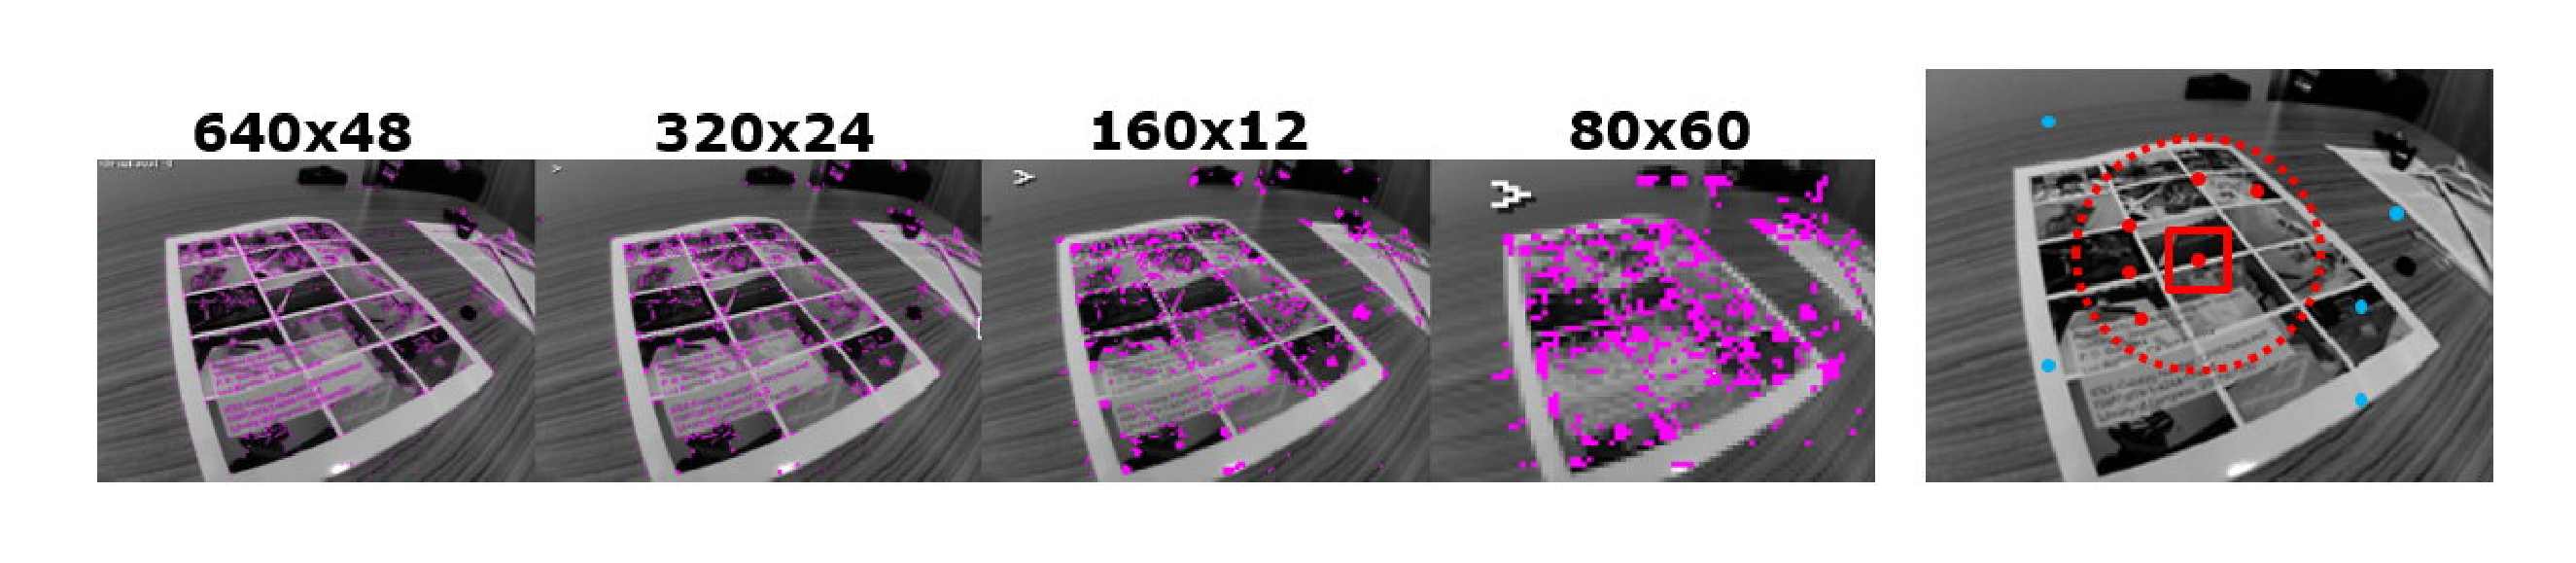
\includegraphics[width=14cm]{PTAM01.pdf}
\caption{视界空间中利用FAST提取特征点和搜索对应特征点示意图,左图表示视界空间的down sampling,以及基于FAST方法的特征点选取,右图为在对应的尺度空间中搜索对应的特征点}
\label{fig:PTAM01}
\end{figure}
在得到所有特征点的信息之后,算法求解以下的优化问题
计算相机姿态的更新(设$P_{t+1}$为当前特征点集合):

\begin{equation}
\label{eq:post_update}
\underset{\mu}{argmin} \sum_{j\in P_{t+1}} \psi( \frac{\lVert\mathbf{e}_j\rVert}{\sigma_j} , \sigma_T)
\end{equation}
\begin{equation}
\mathbf{e}_j= (\hat{u_j},\hat{v_j})- f(exp(\mu)E_{K_{t}\itW} \mathbf{p_j})
\end{equation}

这里 $\psi$ 为 Tukey loss\cite{A86robuststatistics}:

\begin{equation}
\psi(x,c)= 
\begin{cases}
x(1-\frac{x^2}{c^2}) & \text{for }|x|<c \\
0  &  \text{for }|x|>c
\end{cases}
\end{equation}

为了保证算法的稳定性,追踪进程会进行两次:第一次会从三维模型中抽取50个特征点投影匹配,第二次则抽取1000个特征点进行匹配。同时,如果在特征点投影搜索配对的过程中,如果特征点搜索失败的比率大于某一个阈值的话,算法将会判定这一帧失效,并且自动舍弃(这可能是由于抖动,位移量过大特征点不在视界中等多种原因造成)。


\subsection{PTAM管线之二: Mapping}

在追踪进程持续运行的同时,映射进程会根据追踪进程估计的相机姿态,完成关键帧的选取及三维重建的主要任务。为此,算法首先在初始化阶段,需要用户指定视频流中的两帧(第一帧一般为起始帧),单独进行第一次特征点配对。这样做的目的有两个,一方面是为了利用五点法求解相机模型中的固有参数,另一方面是为了先定位特征点到三维空间中作为初始信息。

\subsubsection{关键帧的选择和插入}
在程序进程中,当视频流被读入之后,对于每一帧图像,算法需要判断是否需要把该帧图像加入关键帧集合。判断主要依据是距离上一关键帧的时间和预估的相机距离,以及图像的质量。在选定关键帧之后,根据追踪进程返回的信息,结合上一关键帧的对应特征点信息,定位深度,从而把特征点加入到三维重建模型中。

\subsubsection{利用BA(Bundle Adjustment)校正}
为了消除帧与帧之间的积累误差,映射进程还需要对整体的投影误差和进行一个优化,即所谓的BA。算法对于所有关键帧求解一次优化问题,也会对局部的几个特征点求解局部的优化问题,它们有以下形式:

\begin{equation}
\underset{\{\mu\},\{\mathbf{p}\}}{argmin} = \sum_{i=1}^{N} \sum_{j\in P_i} \psi(\frac{\lVert\mathbf{e}_j\rVert}{\sigma_j},\sigma_T)
\end{equation}

这里的计算将会采用Levenberg-Marquardt BA算法(详见\cite{Hartley2004})。在完成校正之后,新的特征点的三维信息和关键帧信息将作为追踪进程的输入,传入Tracking进程,两个进程在工作的时候将会保持相互的通信,这样最大程度上保证算法运行的流畅度。上述算法的核心过程,在下方\autoref{fig:PTAM_process}中进行了简要的总结。

\newpage
% 流程图定义基本形状
\tikzstyle{startstop} = [rectangle, rounded corners, minimum width=3cm, minimum height=1cm,text centered, draw=black ] %, fill=red!30]
\tikzstyle{io} = [trapezium, trapezium left angle=70, trapezium right angle=110, minimum width=3cm, minimum height=1cm, text centered, draw=black ]%,fill=blue!30]
\tikzstyle{process} = [rectangle, text width=3cm ,minimum width=3cm, minimum height=1cm, text centered, draw=black]%,fill=orange!30]
\tikzstyle{smallprocess} = [rectangle, text width=2cm ,minimum width=2cm, minimum height=1cm, text centered, draw=black]%,fill=orange!30]
\tikzstyle{decision} = [diamond, aspect=2.5, minimum width=1cm, minimum height=1cm, text centered, draw=black]%,fill=green!30]
\tikzstyle{arrow} = [thick,->,>=stealth]

\begin{figure}
\centering
\begin{tikzpicture}[node distance=2cm]

%定义流程图具体形状
\node (Tstart) [startstop] {Tracking};
\node (in1) [process, below of=Tstart] {接收Mapping进程的信息};
\node (pro1) [process, below of=in1] {提取当前帧特征点};
\node (pro2) [process, below of=pro1] {投影匹配特征点};
\node (pro3) [process, below of=pro2] {根据\autoref{eq:post_update}求解相机姿态变化};
%\node (out1) [io, below of=pro2a] {Output};
%\node (stop) [startstop, below of=out1] {Stop};



\node (Mstart) [startstop, right of= Tstart, xshift=7cm] {Mapping};
\node (stereo) [process, above of = Mstart] {初始化};
\node (Mpro1)  [process, below of = Mstart] {关键帧判定与添加};
\node (Mdec1)  [decision, below of = Mpro1, yshift=-0.6cm] {是否全局收敛};
\node (Mpro2)  [smallprocess, left of = Mdec1, xshift=-2cm] {全局BA};
\node (Mdec2)  [decision, below of = Mdec1, yshift=-0.8cm] {是否局部收敛};
\node (Mpro3)  [smallprocess,left of =Mdec2, xshift=-2cm] {局部BA};
\node (Mpro4)  [process, below of =Mdec2] {更新关键帧和深度信息};
%连接具体形状
\draw [arrow](Tstart) -- (in1);
\draw [arrow](in1) -- (pro1);
\draw [arrow](pro1) -- (pro2);
%\draw [arrow](dec1) -- (pro2a);
%\draw [arrow](dec1) -- (pro2b);
%\draw [arrow](dec1) -- node[anchor=east] {yes} (pro2a);
%\draw [arrow](dec1) -- node[anchor=south] {no} (pro2b);
\draw [arrow](pro2) -- (pro3);
%\draw [arrow](pro2a) -- (out1);
%\draw [arrow](out1) -- (stop);
\draw [arrow](pro3) |- +(-2.5,-1) |- (in1);
\draw [arrow](stereo) -- (Mstart);
\draw [arrow](Mstart) -- (Mpro1);
\draw [arrow](Mpro1) -- (Mdec1);

\draw [arrow](Mdec1) -- node[anchor=south] {否} (Mpro2);
\draw [arrow](Mdec1) -- node[anchor=west] {是} (Mdec2);
\draw [arrow](Mdec2) -- node[anchor=west] {是} (Mpro4);
\draw [arrow](Mdec2) -- node[anchor=south] {否} (Mpro3);

\draw [arrow](Mpro2) |- +(0,-1.3) -- +(4,-1.3) -- (Mdec2);
\draw [arrow](Mpro3) |- (Mpro4);

\draw [arrow](Mpro4) -| +(2.5,1) |- (Mpro1);

\draw [arrow](in1) -- node[anchor=north] {匹配特征点对,相机姿态估计} (Mpro1);
\draw [arrow](Mpro1) -- node[anchor=south] {关键帧信息,三维重建模型} (in1);

\end{tikzpicture}

\caption{基于BA的单目经典算法PTAM的流程示意图}
\label{fig:PTAM_process}

\end{figure}


\section{PTAM算法的实际效果}

本节重点比较和讨论对于PTAM算法运行效果。

\subsection{在一般电脑上运行}

我们实现了PTAM在Win10 32bit, openCV 3.2, VS2015的实际环境下,利用笔记本摄像头或者与手机摄像头相连的方式,在一般的笔记本电脑上运行的成果,运行的实际效果如下图所示。对于开放的场景(如寝室内部),实际测试中十分卡顿,掉帧严重,且追踪能力不强。对于特定的平面场景(如桌面),实际测试结果(例如\autoref{fig:PTAMrun})也不近如人意,虽然有时会正确侦测到平面并完成渲染,但有时三维重建和平面的探测结果非常奇怪,十分不鲁棒。。且初始化的stereo init非常依赖初值,可能需要$1\sim5$秒的时间

\begin{figure}[!htbp]
\centering 
\subfloat[实际场景追踪]{
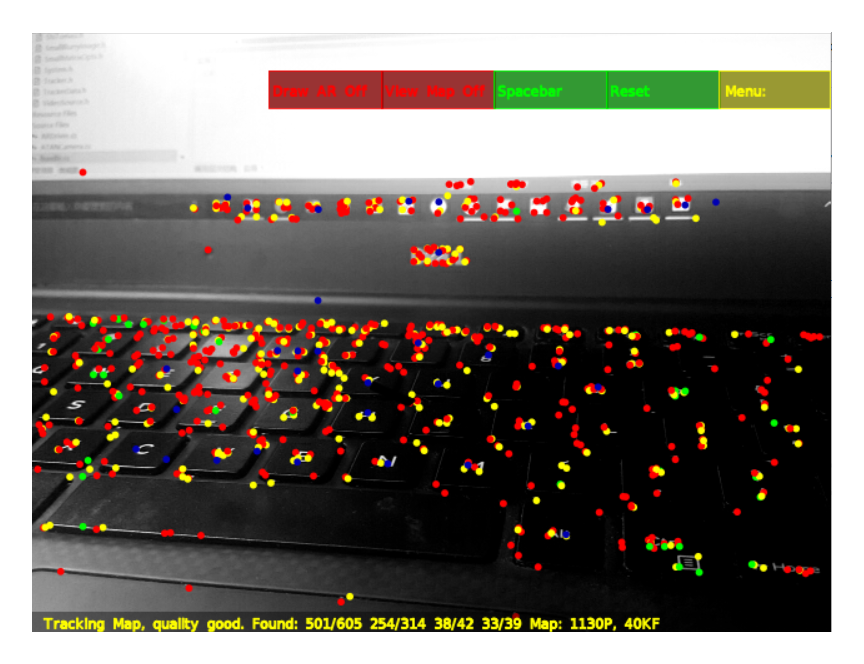
\includegraphics[width=4.5cm]{PTAMrun01.png}}
\subfloat[平面探测与AR渲染]{
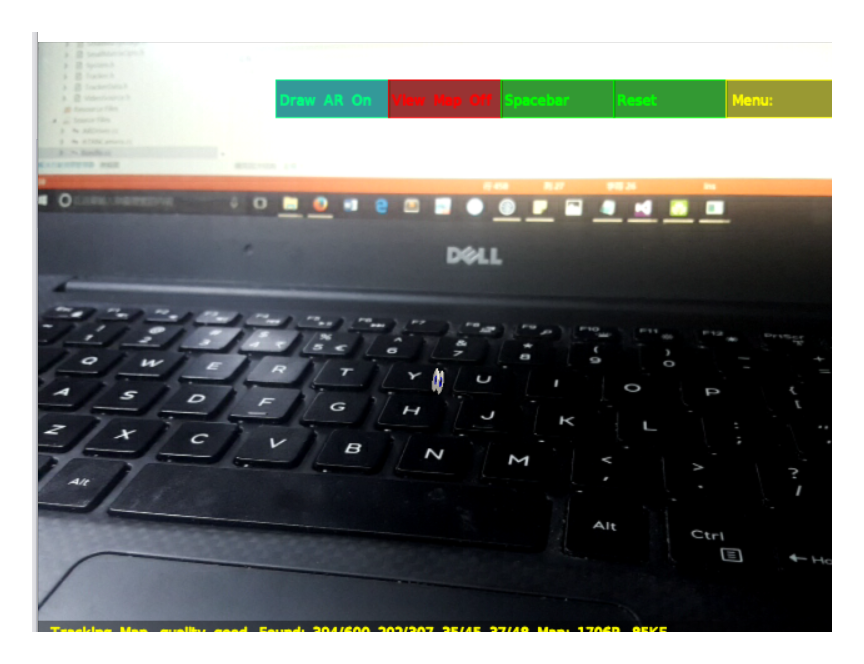
\includegraphics[width=4.5cm]{PTAMrun02.png}}
\subfloat[稀疏三维地图重建]{
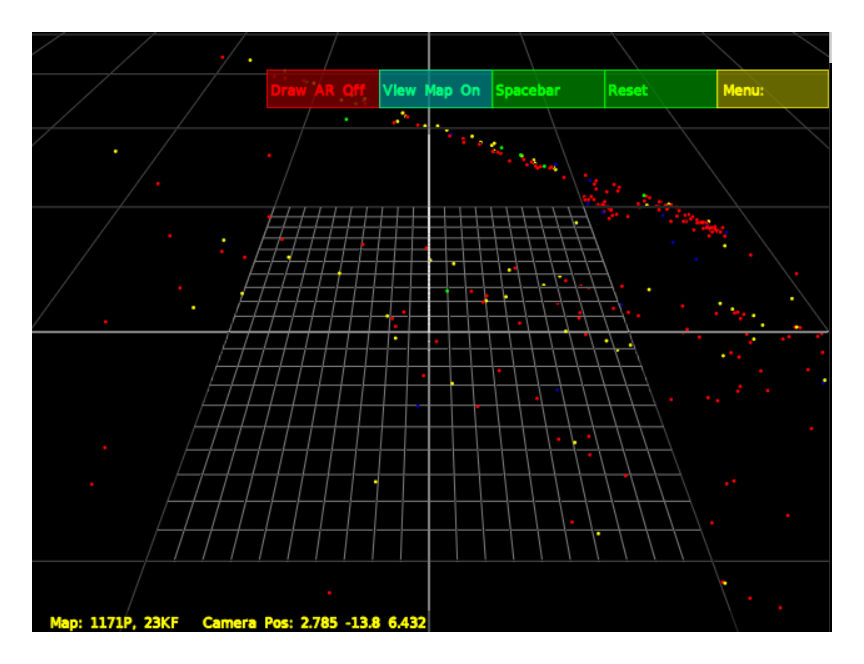
\includegraphics[width=4.5cm]{PTAMrun03.png}}
\caption{PTAM在电脑上实际运行的效果}
\label{fig:PTAMrun}
\end{figure}

\subsection{在智能手机上运行}

智能手机的性能会是制约此类算法在手机上表现的一个重要因素,\cite{Klein2009}中尝试把PTAM的系统移植到Iphone中,得到了\autoref{fig:PTAMcell01}所示的结果。我们虽然并未实现该算法,但可以预见该算法在手机上的运算效率并不会很高。

\begin{figure}[!htbp]
\centering
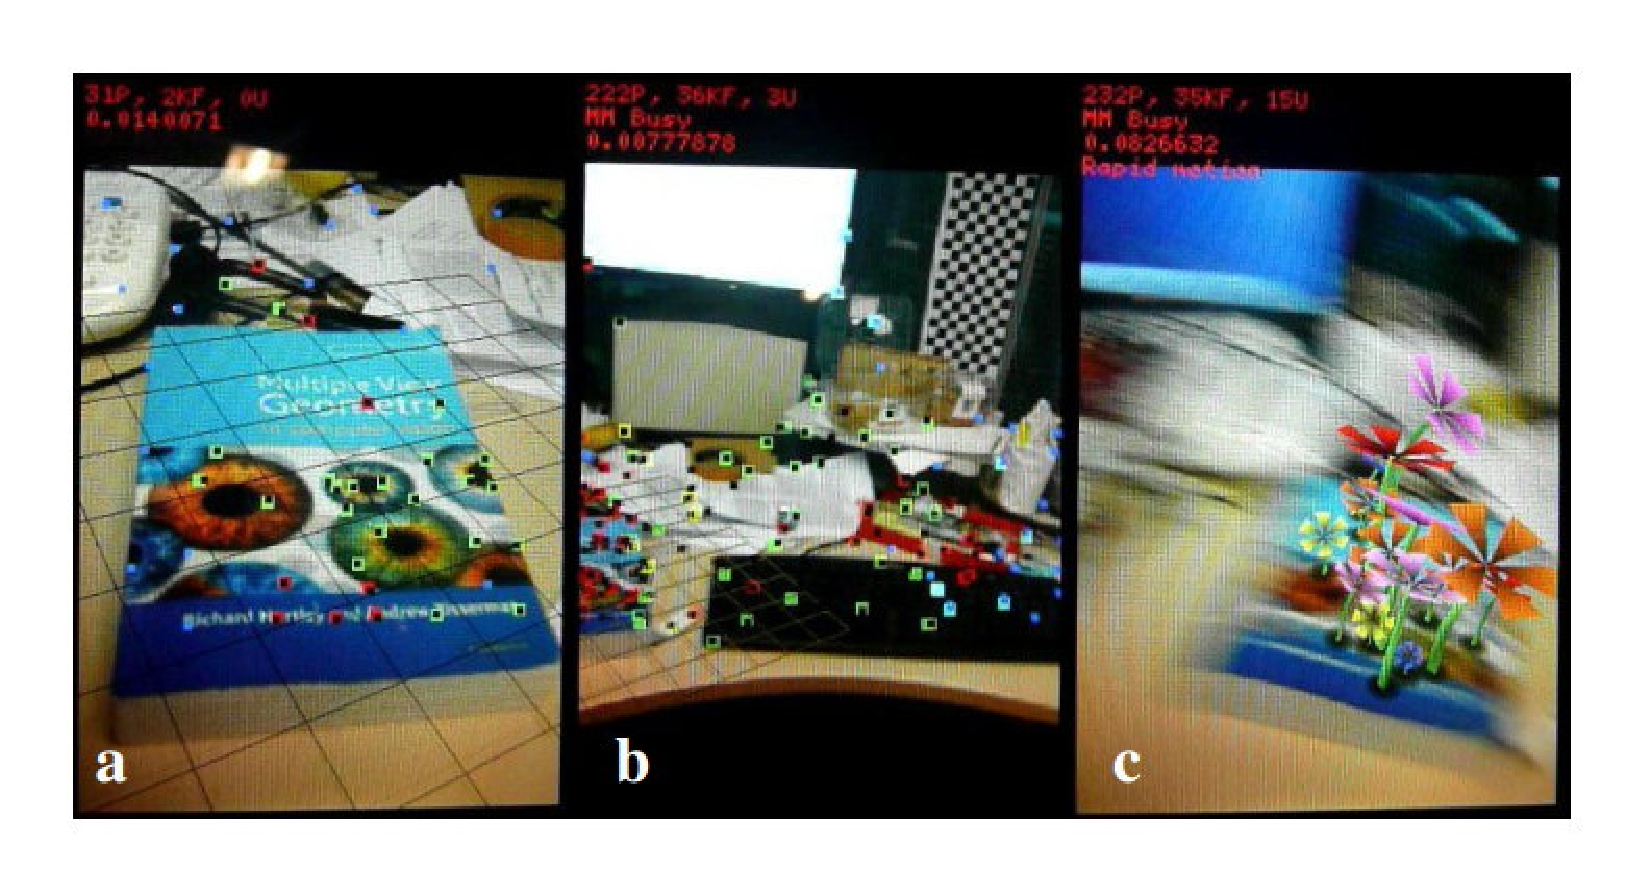
\includegraphics[width=12cm]{PTAMcell01.pdf}
\caption{在智能手机上运行的结果,(a)图为起始状态,(b)图表现了特征点的追踪,(c)图表示了在运动过程中的平面捕捉与AR渲染。由于手机运算能力限制,特征点数量较PC端大幅减少}
\label{fig:PTAMcell01}
\end{figure}

  %\chapter{模板的基础使用说明}

\section{模板基本说明}
使用本模板,您应首先具备基本的\LaTeX 知识,如果您刚刚接触\LaTeX,建议您先学习相关的用户文档或教程。

模板文件名为ustcthesis.cls。方便起见,将该文件放置在与论文主文件同一文件夹中即可。如果需要使用增强功能,模板提供了一个名为ustcxtra.cls的补充包。将该文件放置在与论文主文件同一文件夹中即可。

模板提供一个文档类ustcthesis,使用\verb|\documentclass{ustcthesis}|来加载模板。

模板可以使用ctexbook文档类的相应选项,默认加载的是 cs4size, a4paper, fancyhdr, fntef。需要注意的是默认加载 \emph{双面/章节从奇数页开始} 选项,如果需要\emph{单面} 选项,请使用:
\begin{Code}
\documentclass[<学位>,oneside,openany]{ustcthesis}
\end{Code}

\begin{table}[htp]
\centering
\tabcaption{模板提供的新文档选项}
\label{tab:newdocopt}
\begin{tabular}{lL{5cm}L{4cm}}
\toprule
文档选项&说明&备注\tabularnewline
\midrule
bachelor	&学士				&\multirow{3}{4cm}{指明论文类型,不能同时存在}\tabularnewline
master		&硕士				&\tabularnewline
doctor		&博士				&\tabularnewline
basic		&仅使用基础功能	&此时无法使用增强包中的命令\tabularnewline
oldfontcfg	&使用老版本的硕博论文模板的字体设置			&需要补充包\tabularnewline
euler		&使用euler数学字体&需要补充包\tabularnewline
adobefont	&使用adobe的字体	&\multirow{2}{4cm}{仅仅防止误输入}\tabularnewline
adobefonts	&使用adobe的字体	&\tabularnewline
notchinese	&使用外文撰写论文	Use this option to write thesis in other laguage(s)& If you use language(s) other than Chinese and English, you should refer to \autoref{tab:newcmd}. \tabularnewline
\bottomrule
\end{tabular}
\end{table}

\subsection{模板推荐加载设置}
推荐使用如下选项加载模板:
\begin{Code}
\documentclass[<学位>,euler,twoside,openright]{ustcthesis}
\end{Code}

如果缺少大多数宏包,建议使用
\begin{Code}
\documentclass[<学位>,basic,twoside,openright]{ustcthesis}
\end{Code}

\section{模板提供的新环境和命令}
模板提供了若干个新环境和命令,如\autoref{tab:newenv}和\autoref{tab:newcmd}所列,这些新环境和命令有的比较简单,有的则附有对应的示例。

\begin{longtable}{lll}%@{\extracolsep{\fill}}
\caption[模板提供的新环境]{模板提供的新环境}
\label{tab:newenv} \\
\toprule
名称  & 说明 & 备注\tabularnewline\midrule
\endfirsthead
\bottomrule
\endfoot
\caption[模板提供的新环境(续)]{模板提供的新环境(续)} 
\label{tab:newenv2} \\
\toprule
名称  & 说明 & 备注\tabularnewline\midrule
\endhead
\bottomrule
\endlastfoot
enabstract&英文摘要&\tabularnewline
cnabstract&中文摘要&\tabularnewline
thanks&致谢&\tabularnewline
denotation&主要符号对照表&需要ustcxtra,用法见./chapter/denotation.tex\tabularnewline
Code&代码&需要ustcxtra,效果见\autoref{codex}\tabularnewline
Codex&代码&需要ustcxtra,效果见\autoref{codex}\tabularnewline
CodeScript&代码&需要ustcxtra,效果见\autoref{codex}\tabularnewline
CodexScript&代码&需要ustcxtra,效果见\autoref{codex}\tabularnewline
code&代码&需要ustcxtra,效果未测试\tabularnewline
theorem &定理&\tabularnewline
lemma &引理&\tabularnewline
example &例&\tabularnewline
algorithm &算法&\tabularnewline
definition &定义& \tabularnewline
axiom &公理 &\tabularnewline
property &性质 & \tabularnewline
proposition &命题 &\tabularnewline
corollary& 推论 &\tabularnewline
remark &注解  &\tabularnewline
condition &条件 & \tabularnewline
conclusion &结论 & \tabularnewline
assumption &假设 & \tabularnewline
prove &证明 &\tabularnewline
proof&证明 &与prove的区别见\autoref{pic:proofandprove}\tabularnewline
\end{longtable}

\begin{longtable}{lp{0.35\textwidth}p{0.35\textwidth}}%@{\extracolsep{\fill}}
\caption[模板提供的新命令]{模板提供的新命令}
\label{tab:newcmd} \\
\toprule
名称  & 说明 & 备注\tabularnewline\midrule
\endfirsthead
\bottomrule
\endfoot
\caption[模板提供的主要新命令(续)]{模板提供的主要新命令(续)} 
\label{tab:newcmd2} \\
\toprule
名称  & 说明 & 备注\tabularnewline\midrule
\endhead
\bottomrule
\endlastfoot
\textbackslash chuhao\{\}&字号:初号&类似的有:\textbackslash yihao\{\}...\textbackslash qihao\{\}\tabularnewline
\textbackslash xiaochu\{\}&字号:小初号&类似的有:\textbackslash xiaoer\{\}...\textbackslash xiaowu\{\}\tabularnewline
\textbackslash xiaochuhao\{\}&字号:小初号&类似的有:\textbackslash xiaoerhao\{\}...\textbackslash xiaowuhao\{\}\tabularnewline
\textbackslash ustclofname\{\}&定义图表索引名称&需在\textbackslash ustclof前使用\tabularnewline
\textbackslash ustclof&生成图表索引并加入目录&\tabularnewline
\textbackslash ustclotname\{\}&表格索引名称&与\textbackslash ustclofname\{\}类似\tabularnewline
\textbackslash ustclot&表格索引&与\textbackslash ustclot类似\tabularnewline
\textbackslash ustcloaname\{\}&算法索引名称&需要ustcxtra,与\textbackslash ustclofname\{\}类似\tabularnewline
\textbackslash ustcloa&算法索引&需要ustcxtra,与\textbackslash ustclof类似\tabularnewline
\textbackslash title\{\}&标题&中文\tabularnewline
\textbackslash author\{\}&作者&中文\tabularnewline
\textbackslash advisor\{\}&导师&中文\tabularnewline
\textbackslash coadvisor\{\}&第二导师&中文,可留空\tabularnewline
\textbackslash major\{\}&专业&硕博全称,本科不需要\tabularnewline
\textbackslash depart\{\}&院系&硕博代号,本科全称\tabularnewline
\textbackslash submitdate\{\}&完成日期&中文\tabularnewline
\textbackslash en...\{\}&由title至submitdate&以上命令的英文版本\tabularnewline
\textbackslash studentid\{\}&学号&仅本科需要\tabularnewline
\textbackslash spinetitle\{\}&书脊使用的标题&在\textbackslash title中含有部分控制命令时使用\tabularnewline
\textbackslash covertitle\{\}&封皮使用的中文标题&在\textbackslash title超过两行或其他情况时使用\tabularnewline
\textbackslash coverentitle\{\}&封皮使用的英文标题&仅本科需要,在\textbackslash entitle超过三行或其他情况时使用\tabularnewline
\textbackslash makecover[][]&生成制本厂规定格式的封皮&详细用法见main.tex文件中注释\tabularnewline
\textbackslash keywords\{\}&中文关键词&在cnabstract中使用\tabularnewline
\textbackslash enkeywords\{\}&英文关键词&在enabstract中使用\tabularnewline
\textbackslash figcaption\{\}&图形标题&无论是否在图形环境中均可得到正确标题\tabularnewline
\textbackslash tabcaption\{\}&&与上类似,表格用\tabularnewline
C\{width\}&定宽居中&表格环境中p\{width\}的加强,参考\autoref{tab:tblcmp}\tabularnewline
L\{width\}&定宽左齐&\tabularnewline
R\{width\}&定宽右齐&\tabularnewline
\textbackslash scite\{\}&上标引用&\tabularnewline
\textbackslash song&宋体&另有其他,详见ustcxtra\tabularnewline
\textbackslash upGamma&立直希腊Gamma&另有其他,详见ustcxtra\tabularnewline

\textbackslash otherustcstr  & 'University of Science and Technology of China'. A translation of this string in your own language. \emph{Only useful when you are writting a thesis in language(s) other than Chinese and English}. &  According to regulations of USTC, your need to put three title pages: Chinese, English and your own language title pages. So use these commands to generate the third title page. \tabularnewline%
\textbackslash otherthesisstr  & 'A dissertation for bachelor(/master/doctor)'s degree' & Similar to previous one \tabularnewline%
\textbackslash otherauthorstr  & 'Author' & Similar to previous one \tabularnewline%
\textbackslash otherdepartmentstr  & 'Department' & Similar to previous one \tabularnewline%
\textbackslash otherstudentidstr  & 'Student ID' & Similar to previous one \tabularnewline%
\textbackslash othersupervisorstr  & 'Supervisor' & Similar to previous one \tabularnewline%
\textbackslash otherfinishedtimestr  & 'Finished Time' & Similar to previous one \tabularnewline%
\textbackslash otherspecialitystr  & 'Speciality' & Similar to previous one \tabularnewline%
\textbackslash othertitle  & Thesis title. Put your thesis title in your own language here. \emph{Only useful when you are writting a thesis in language(s) other than Chinese and English}. &   \tabularnewline
\textbackslash otherauthor  & Your name & Similar to previous one \tabularnewline
\textbackslash otheradvisor  & Your advisor's name & Similar to previous one \tabularnewline
\textbackslash othercoadvisor  & Co-advisor & Similar to previous one \tabularnewline
\textbackslash othersubmitdate  & Thesis submit date & Similar to previous one \tabularnewline
\textbackslash othermajor  & Your major & Similar to previous one \tabularnewline
\textbackslash otherdepart  & Your department & Similar to previous one \tabularnewline
\end{longtable}

需要注意的是,这里prove环境翻译为“证明”,事实上,其实prove环境不是用作theorem等类似环境配套证明的,prove环境是与theorem等环境同级别的环境。与theorem等环境相配套的证明环境是proof环境。使用时请注意下两个环境的差异:proof环境是没有编号的,是与theorem这类环境配合使用的;prove环境是有编号的,更多的是类似于证明题的题目。详细的差别见\autoref{pic:proofandprove}。

\begin{figure}
\centering
  \framebox{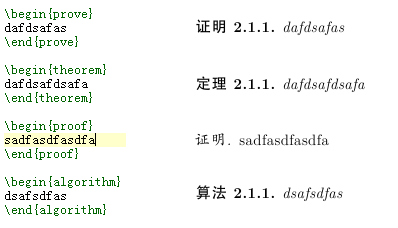
\includegraphics[scale=1]{figures/proofandprove}}
  \figcaption{proof、prove以及部分其他数学环境的差异}
  \label{pic:proofandprove}
\end{figure}

\section{使用模板的一些建议}

公式、章节、图和表格等(不包括脚注和参考文献)的交叉引用可以使用\verb|\autoref{label}|来得到正确的引用。例如使用\verb|\autoref{some_pic}|可以得到“图 X”的引用,使用\verb|\autoref{some_table}|可以得到“表 X”的引用。

建议使用\verb|\figcaption{}|命令得到所有图形的标题,表格也是。这样无论是否在图形环境中均能够得到正确的带图/表编号的标题,而在图形环境之外使用\verb|\caption{}|命令会报错。

%封面是按照制本厂的要求制作的,其中行宽和行高都是固定的,中文标题最多占两行,英文标题最多占三行。如果您的题目超过了这个限制,请缩减题目长度,不要擅自修改模板中的相关配置参数。


  %
\chapter{代码示例}
\label{chap:example}
\section{Euler数学字体示例}
$$
abcdefghijklmnopqrstuvwxyz
$$
$$
ABCDEFGHIJKLMNOPQRSTUVWXYZ
$$
$$
0123456789
$$
\begin{equation}
\begin{split}
\{S_i=0\}=\frac{a_i}{b_i+a_i} \\
\{S_i=1\}=\frac{b_i}{b_i+a_i} \label{1}
\end{split}
\end{equation}

\section{上标引用示例}
\verb|\scite{lshort-cn}|,效果\scite{lshort-cn}。

\section{表格环境加强命令示例}
本模板提供了表格环境下p\{width\}加强版命令,使用L\{width\}等可以在指定宽度的同时指定对齐方式。

\begin{minipage}{\textwidth}
\begin{Codex}[numbers=left]
\begin{table}
\tabcaption{几种命令效果对比的对比}
\label{tab:tblcmp}
\centering
\begin{tabular}{c||l|c|r|p{2.5cm}|L{2.5cm}|C{2.5cm}|R{2.5cm}}
\hline
命令&l&c&r&p\{width\}&L\{width\}&C\{width\}&R\{width\}\\
\hline
效果&左齐&居中&右齐&定宽&左齐定宽&居中定宽&右齐定宽\\
\hline
\end{tabular}
\end{table}
\end{Codex}

\tabcaption{几种命令效果对比的对比}
\label{tab:tblcmp}
\centering
\begin{tabular}{c||l|c|r|p{2.5cm}|L{2.5cm}|C{2.5cm}|R{2.5cm}}
\hline
命令&l&c&r&p\{width\}&L\{width\}&C\{width\}&R\{width\}\\
\hline
效果&左齐&居中&右齐&定宽&左齐定宽&居中定宽&右齐定宽\\
\hline
\end{tabular}
\end{minipage}

\section{自定义代码环境示例}
\label{codex}
\subsection{Code环境}
\begin{minipage}{\textwidth}
\begin{minipage}{0.4\textwidth}
\begin{Code}[label=a.cpp, numbers=left]
This is Code environment
A simple example.
For more options, see fancyvrb's manual.
\end{Code}
\end{minipage}
\hfill\begin{minipage}{0.4\textwidth}
\begin{Verbatim}[fontsize=\scriptsize,baselinestretch=0.9,xleftmargin=3mm,frame=lines,labelposition=all,framesep=5pt]
\begin{Code}[label=a.cpp, numbers=left]
This is Code environment
A simple example.
For more options, see fancyvrb's manual.
\end{Code}
\end{Verbatim}
\end{minipage}
\end{minipage}

\subsection{Codex环境}
\begin{minipage}{\textwidth}
\begin{minipage}{0.4\textwidth}
\begin{Codex}[label=a.cpp, numbers=left]
This is Codex environment
A simple example.
For more options, see fancyvrb's manual.
\end{Codex}
\end{minipage}
\hfill\begin{minipage}{0.4\textwidth}
\begin{Verbatim}[fontsize=\scriptsize,baselinestretch=0.9,xleftmargin=3mm,frame=lines,labelposition=all,framesep=5pt]
\begin{Codex}[label=a.cpp, numbers=left]
This is Codex environment
A simple example.
For more options, see fancyvrb's manual.
\end{Codex}
\end{Verbatim}
\end{minipage}
\end{minipage}

\subsection{CodeScript环境}
\begin{minipage}{\textwidth}
\begin{minipage}{0.4\textwidth}
\begin{CodeScript}[label=a.cpp, numbers=left]
This is CodeScript environment
A simple example.
For more options, see fancyvrb's manual.
\end{CodeScript}
\end{minipage}
\hfill\begin{minipage}{0.4\textwidth}
\begin{Verbatim}[fontsize=\scriptsize,baselinestretch=0.9,xleftmargin=3mm,frame=lines,labelposition=all,framesep=5pt]
\begin{CodeScript}[label=a.cpp, numbers=left]
This is CodeScript environment
A simple example.
For more options, see fancyvrb's manual.
\end{CodeScript}
\end{Verbatim}
\end{minipage}
\end{minipage}

\subsection{CodexScript环境}
\begin{minipage}{\textwidth}
\begin{minipage}{0.4\textwidth}
\begin{CodexScript}[label=a.cpp, numbers=left]
This is CodexScript environment
A simple example.
For more options, see fancyvrb's manual.
\end{CodexScript}
\end{minipage}
\hfill\begin{minipage}{0.4\textwidth}
\begin{Verbatim}[fontsize=\scriptsize,baselinestretch=0.9,xleftmargin=3mm,frame=lines,labelposition=all,framesep=5pt]
\begin{CodexScript}[label=a.cpp, numbers=left]
This is CodexScript environment
A simple example.
For more options, see fancyvrb's manual.
\end{CodexScript}
\end{Verbatim}
\end{minipage}
\end{minipage}

\section{表格示例}
具体代码请参考源文件./chapter/chap-example.tex。
\begin{table}[htbp]
\centering
\caption{基于因子分析的失配补偿结果}
\label{tab:jfa-gmm-ubm}
\begin{tabular}{cccccc}
    \toprule
    &\multirow{2}{*}{\#Mix}&\multicolumn{2}{c}{No-norm}
    &\multicolumn{2}{c}{Tnorm}\\
    \cline{3-4} \cline{5-6}
		&		& EER(\%) 	& MinDCF & EER(\%) 	& MinDCF\\
    \midrule
	\multirow{3}{*}{GMM-UBM}
    &256 		& 12.43 	& 0.0647	& 12.85    & 0.0580\\
    &512 		& 10.02 	& 0.0464	& 8.88 	   & 0.0370\\
    &1024 		& 9.97 	    & 0.0457	& 8.72 	   & 0.0372\\
    \midrule
	\multirow{3}{*}{Factor Analysis}
    &256 		& 8.09 	& 0.0331 	& 7.39 	& 0.0319\\
    &512 		& 7.08 	& 0.0305 	& 6.53 	& 0.0292\\
    &1024 		& 6.83 	& 0.0295 	& \textbf{6.29} 	& \textbf{0.0279}\\
 \bottomrule
\end{tabular}
\end{table}

\section{算法示例}
具体代码请参考源文件./chapter/chap-example.tex。
\IncMargin{1em}
\begin{algorithm}
\SetKwData{Left}{left}\SetKwData{This}{this}\SetKwData{Up}{up}
\SetKwFunction{Union}{Union}\SetKwFunction{FindCompress}{FindCompress}
\SetKwInOut{Input}{input}\SetKwInOut{Output}{output}
\Input{$O_t,UBM,U$}
\Output{$x,y$}
\BlankLine
\emph{$y\leftarrow 0;$$x_h\leftarrow 0;$$h=1,...,H$ }\;
\For{$i=1$ \KwTo Number of E-M iterations}{
\emph{E Step}:\\
\For{$h=1$ \KwTo $H$}{\label{forins}
对于每一条语音段,计算其EM统计量(零阶统计量$N_h$,一阶统计量$S_{X,h}$\;
}
计算每一个人所有语音段的零阶统计量$N$\\
计算每一个人所有语音段的一阶统计量$S$\\
\emph{M Step}:\\
\For{$j=1$ \KwTo Number of Gauss-Seidel iterations}{
\For{$h=1$ \KwTo $H$}{\label{forins}
估计每一语音段$h$的失配因子$x_h$
}
估计模型的话者因子$y$
}
}
\Return{$\mu = m+Dy$}
\caption{disjoint decomposition}\label{algo_disjdecomp}
\end{algorithm}\DecMargin{1em}

\section{引用参考文献示例}
参考文献测试:\citep{deng:01a}
  %自行添加
  %\include{chapter/...}

%%%%%%%%%%%%%%%%%%%%%%%%%%%%%%
%% 附件部分
%%%%%%%%%%%%%%%%%%%%%%%%%%%%%%
\backmatter

  % 参考文献
  % 使用 BibTeX
  % 选择参考文献的排版格式。注意ustcbib这个格式不保证完全符合要求,请自行决定是否使用
  \bibliographystyle{ustcbib}%{GBT7714-2005NLang-UTF8}
  \bibliography{bib/tex}
  \nocite{*} % for every item
  % 不使用 BibTeX
  % %\renewcommand{\baselinestretch}{0.5}
\begin{thebibliography}{10}

\bibitem{deng:01a}
{邓建松,~彭冉冉,~陈长松邓建松,~彭冉冉,~陈长松邓建松,~彭冉冉,~陈长松邓建松,~彭冉冉,~陈长松邓建松,~彭冉冉,~陈长松邓建松,~彭冉冉,~陈长松邓建松,~彭冉冉,~陈长松邓建松,~彭冉冉,~陈长松邓建松,~彭冉冉,~陈长松邓建松,~彭冉冉,~陈长松邓建松,~彭冉冉,~陈长松}.
\newblock {\em \LaTeXe{}~科技排版指南}.
\newblock 科学出版社,~书号:~7-03-009239-2/TP.1516, 北京, 2001.

\bibitem{wang:00a}
王磊.
\newblock {\em \LaTeXe{}~插图指南}.
\newblock 2000.

\bibitem{zhang:03a}
张林波.
\newblock {\em 关于新版~CCT~的说明}.
\newblock 2003.

\bibitem{lshort-cn}
C\TeX{} 翻译小组.
\newblock {\em lshort~中文版~3.20}.
\newblock 2003.

\bibitem{knuth86e}
Donald~E. Knuth.
\newblock {\em Computer Modern Typefaces}, volume~E of {\em Computers and
  Typesetting}.
\newblock Addison-Wesley, Reading, Massachusetts, 1986.

\bibitem{knuth86d}
Donald~E. Knuth.
\newblock {\em {METAFONT}: The Program}, volume~D of {\em Computers and
  Typesetting}.
\newblock Addison-Wesley, Reading, Massachusetts, 1986.

\bibitem{knuth86c}
Donald~E. Knuth.
\newblock {\em The {METAFONT}book}, volume~C of {\em Computers and
  Typesetting}.
\newblock Addison-Wesley, Reading, Massachusetts, 1986.

\bibitem{knuth86b}
Donald~E. Knuth.
\newblock {\em {TeX}: The Program}, volume~B of {\em Computers and
  Typesetting}.
\newblock Addison-Wesley, Reading, Massachusetts, 1986.

\bibitem{knuth86a}
Donald~E. Knuth.
\newblock {\em The {TeX}book}, volume~A of {\em Computers and Typesetting}.
\newblock Addison-Wesley, Reading, Massachusetts, 1986.

\bibitem{lamport85a}
Leslie Lamport.
\newblock {\em {LaTeX} --- A Document Preparation System: User's Guide and
  Reference Manual}.
\newblock Addison-Wesley, Reading, Massachusetts, 2nd edition, 1985.


\end{thebibliography}


  % 附录,没有请注释掉
  \begin{appendix}
    
\chapter{中国科学技术大学研究生学位论文撰写规范}
\label{chap:requires}
\section*{以下文字仅作示例,一切以学校规定为准!}
研究生院规定在此下载\url{http://gradschool.ustc.edu.cn/ylb/material/xw/wdxz/1.doc}

研究生学位论文集中反映研究生在研究工作中所取得的成果,代表研究生研究工作的水平,也是申请和授予相应学位的主要依据。为提高研究生学位论文的撰写质量,做到学位论文在内容和格式上的规范化,我们编写了《中国科学技术大学研究生学位论文撰写规范》,供申请学位的研究生参考执行。其中参考文献著录规则我们根据GB/T 7714-2005的标准撰写。硕士和博士学位论文除在研究深度等方面要求不同外,撰写要求基本一致。

\section{内容要求}

\subsection{封面} 
采用研究生院规定的统一封面,封面包含内容如下: 
\subsubsection{密级} 涉密论文必须在论文封面标注密级(内部、秘密、机密),同时注明保密年限。
\subsubsection{论文题目} 应准确概括整个论文的核心内容,简明扼要,最多不超过30字,必要时可以加副标题。
\subsubsection{作者姓名} 英文封面中按英文习惯书写,即名在前。姓名需写全拼。
\subsubsection{学科专业} 写所在专业的全称,不可用简写。
\subsubsection{导师姓名} 一般允许有两名指导教师,主要指导教师姓名写在第一位,后附其职称,次要指导教师排第二位,也需注明职称。
\subsubsection{完成时间} 填写论文打印成文的年月日。

\subsection{中国科学技术大学学位论文原创性和授权使用声明}
本部分内容使用统一的模版,具体内容见格式范例,提交时作者须亲笔签名。

\subsection{摘要和关键词}
\subsubsection{中文摘要}
摘要是论文内容的总结概括,应简要说明论文的研究目的、基本研究内容、研究方法、创新性成果及其理论与实际意义,突出论文的创新之处。不宜使用公式、图表,不标注引用文献。 
\subsubsection{中文关键词} 
关键词是为了文献标引工作从论文中选取出来用以表示全文主题内容信息的单词和术语,一般3--8个词,要求能够准确概括论文的核心内容。
\subsubsection{英文摘要与关键词}
以中文书写的论文,内容与中文摘要和关键词完全一致,其他语种书写的论文以简略为原则,不需要相同。

\subsection{目录}
目录页由论文的章、条、附录等序号、名称和页码组成。论文中如图表较多,可以分别列出清单置于目次页之后。图的清单应有序号、图题和页码。表的清单应有序号、表题和页码。

\subsection{符号说明}
如果论文中使用了大量的物理量符号、标志、缩略词、专门计量单位、自定义名词和术语等,应编写成注释说明汇集表。若上述符号等使用数量不多,可以不设此部分,但必须在论文中出现时加以说明。

\subsection{正文}
正文是学位论文的主体,包括绪论、论文主体及结论等部分。
\subsubsection{绪论}
内容应包括:选题的背景和意义,文献综述及研究现状,研究内容与预期结果,研究方法和实验设计,论文结构安排等。要求实事求是,不夸大、缩小前人的工作和自己的工作,言简意赅,突出重点,不与摘要雷同。
\subsubsection{论文主体}
论文主体是正文的核心部分,占主要篇幅,它是将学习、研究和调查过程中筛选、观察和测试所获得的材料,经过加工整理和分析研究,由材料而形成论点。由于各学科及具体选题的差异,此部分不作统一规定。但总体内容必须实事求是,客观真切,准确完备,合乎逻辑,层次分明,简练可读。
\subsubsection{结论}
结论是对整个论文主要成果的总结,应明确、精炼、完整、准确。其中应明确指出本研究的创新点,对论文的学术价值和应用价值等加以预测和评价,说明研究中尚难解决的问题并提出今后进一步在本研究方向进行研究工作的设想或建议。

\subsection{参考文献}
本着以严谨求实的科学态度撰写论文,凡学位论文中有引用或参考、借用他人成果之处,均应详细列出所引文献的名称、作者、发表刊物、发表时间、卷号、页码等,严禁抄袭剽窃。  
\subsection{附录}
主要列入正文内过分冗长的公式推导,供查读方便所需的辅助性数学工具或表格,重复性数据图表,论文使用的缩写,程序全文及说明等。

\subsection{致谢}
对给予各类资助、指导和协助完成研究工作以及提供各种对论文工作有利条件的单位及个人表示感谢。致谢应实事求是,切忌浮夸与庸俗之词。

\subsection{在读期间发表的学术论文与取得的其他研究成果}
按学术论文发表的时间顺序,列齐本人在攻读学位期间发表或已录用的学术论文清单(发表刊物名称、卷册号、页码、年月及论文署名、作者排序)。其他研究成果可以是申请的专利、获得的奖项及完成的项目等。
 
\section{书写规定}

\subsection{论文的字数要求}
硕士学位论文要求不少于3万字,博士学位论文要求不少于5万字。

\subsection{文字、标点符号和数字}
除留学生和外语专业研究生外,学位论文一律用汉字书写。除非特殊需要,不得使用已废除的繁体字、异体字等不规范汉字。标点符号的用法以GB/T 15834—1995《标点符号用法》为准。数字用法以GB/T 15835—1995《出版物上数字用法的规定》为准。

留学生的学位论文所采用语种可以和导师商定,但论文封面须用中文。

\subsection{封面与扉页}
\subsubsection{秘级} 封面的秘级可以标注为内部、秘密和机密,各密级的保密时限分别为小于等于5年、小于等于10年和小于等于20年,非保密论文不标注密级。
\subsubsection{题目} 题目中避免使用缩略词、首字母缩写字、字符、代号和公式等。
\subsubsection{日期} 封面的日期用汉字书写。
\subsubsection{扉页} 扉页的内容与封面一致。扉页后,需给出英文的封面。其他语种书写的论文还需在英文封面后附上正文所用语种书写的封面。

\subsection{目录}
目录应包括论文的全部内容,包括中英文摘要和附录等,正文章节题名要求编到第3级标题,即×.×.×。一级标题顶格书写,二级标题缩进一个汉字符位置,三级标题缩进两个汉字符位置。

\subsection{摘要与关键词}
\subsubsection{摘要}
摘要分中文和英文两种,中文在前,英文在后。标题摘要二字中间空一格。摘要的字数,硕士学位论文建议1000字以内,博士学位论文建议3000字以内。留学生用其他语种撰写学位论文时,中文摘要应不少于6000汉字。摘要中不得出现图片、图表、表格或其他插图材料。英文摘要与中文摘要应完全一致。
\subsubsection{关键词}
关键词以显著的字符另起一行并隔行排列于摘要下方,左顶格。中文关键词间空一格,英文关键词间用逗号隔开。

\subsection{论文正文}
\subsubsection{章节及各章标题}
论文正文分章节撰写,每章应另起一页。

各章标题字数一般应在15字以内,不使用标点符号。标题中尽量不采用英文缩写词,对必须采用者,应使用本行业的通用缩写词。
\subsubsection{序号}
\paragraph{标题序号}
论文标题分层设序。层次以少为宜,根据实际需要选择。各层次标题一律用阿拉伯数字连续编号;不同层次的数字之间用小圆点“.”相隔,末位数字后面不加点号,如“1”,“1.1”,“1.1.1”等;各层次的序号均左起顶格排,后空1个字距接排标题。例如:

第1章 ××××(大标题) 

1.1 ××××(一级节标题)

1.1.1 ××××(二级节标题)

1.1.1.1 ××××(根据需要,也可设三级节标题)

第2章 ××××(大标题)

2.1 ××××(一级节标题)

2.1.1 ××××(二级节标题)

\paragraph{图表等编号} 
论文中的图、表、附注、公式、算式等,一律用阿拉伯数字分章依序连续编码。其标注形式应便于互相区别,如:图 l.1(第1章第一个图)、图2.2(第二章第二个图);表3.2(第三章第二个表)等。
\paragraph{页码}
页码从绪论开始按阿拉伯数字(1,2,3……)连续编排,此前的部分(中英文摘要、目录等)用大写罗马数字(I,II,III…)单独编排,页码位置居于页脚居中。封面、扉页、创新性声明等不编页码。
\subsubsection{页眉}
页眉从中文摘要开始,内容与该部分的一级标题相同,奇偶页相同,各部分的首页也需有页眉。
\subsubsection{名词和术语}
科技名词术语及设备、元件的名称,应采用国家标准或部颁标准中规定的术语或名称。标准中未规定的术语要采用行业通用术语或名称。全文名词术语必须统一。一些特殊名词或新名词应在适当位置加以说明或注解。

采用英语缩写词时,除本行业广泛应用的通用缩写词外,文中第一次出现的缩写词应该用括号注明英文原词。
\subsubsection{量和单位}
量和单位要严格执行GB 3100~3102-93(国家技术监督局1993-12-27发布,1994-07-01实施)有关量和单位的规定。

量的符号一般为单个拉丁字母或希腊字母,并一律采用斜体(pH例外)。为区别不同情况,可在量符号上附加角标。 

在表达量值时,在公式、图、表和文字叙述中,一律使用单位的国际符号,且无例外地用正体。单位符号与数值间要留适当间隙。具体可参见下列表达式3.1。

\subsubsection{图和表}
\paragraph{图}
图应具有“自明性”,即只看图、图题和图例,不阅读正文,就可理解图意。每一图应有简短确切的题名,连同图号置于图下。

图的位置在相关说明文字之后,随文排。坐标比例不宜过大,同一图上不同曲线的点要分别用不同形状的标识符标出。图中的术语、符号、单位等应与正文表述中所用一致。

图题应简明。图号和图题间空1个字符位置,居中排于图的下方。

必要时,应将图上的符号、标记、代码,以及实验条件等,用最简练的文字,横排于图题下方,作为图例说明(图注)。

\paragraph{表}
表的位置也在相应说明文字之后,随文排。表中参数应标明量和单位的符号。表应有自明性。每一表应有简短确切的题名,连同表号置于表上,表号与表题间空一个字符位置。表号用阿拉伯数字分章编号,如第3章第2个表的表号表示为“表3.2”。

表格太大需要转页时,需要在续表上方注明“续表”,表头也应重复排出。

必要时应将表中的符号、标记、代码,以及需要说明事项,以最简练的文字,横排于表题下,作为表注。相关要求同于图注。

\subsubsection{表达式}
表达式主要指数字表达式,也包括文字表达式。表达式需另行起排,原则上应居中,用阿拉伯数字分章编号。序号加圆括号,右顶格排。例如,第3章第1个表达式:

较长的式如必须转行,只能在+,-,×,÷,<,>处转行,序号编于最后一行的最右边。

\subsection{参考文献}
参考文献参照GB/T 7714-2005《文后参考文献著录规则》执行。推荐使用著者-出版年制,即在正文引用文献处标注著者姓名与出版年份,在文后的参考文献表中标注参考文献的详细信息。
\subsubsection{著者-出版年制在正文中的标注方式}

正文中的标注方式分两种:其一,正文里已出现著作者姓名的,在其后用圆括号附上出版年份即可;其二,正文里仅提及有关的资料内容而未提到著作者,则在相应文句处用圆括号标注著作者姓名和出版年份,两者之间加逗号。

例如:

Park et al(1995)根据Laurentia西缘放射状基性岩墙的研究以及与地幔柱有关的澳大利亚Gairdner岩墙群的研究,首次提出约780Ma地幔柱导致Rodinia超大陆的裂解。

其中关于成冰系顶底界时限和冰川活动年龄、超大陆裂解的起始时间和持续时间……是当前中国地球科学界十分活跃并得到迅速发展的研究领域(王平,2003)。

引用同一著者在同一年份出版的多篇文献时,在出版年份之后用英文小写字母a、b、c……区别。如:(王平,2005a);(王平,2005b)

多处引用同一著者的同一文献时,在“()”外以角标的形式著录引文页码。引用有两个以上同姓的著者的外文文献时,则著者要加名字的缩写,但不必加缩写点。

引用多位著者的文献时,对欧美著者只需标注第一个著者的姓,其后附“et al”,仅两位作者的也可全部注出,中间用“and”;对中国著者应该标注第一著者的姓名,其后附“等”字,姓名与“等”字之间留1个空格。例如:……(王平 等,2005) ……。

同一处引用多篇文献时,按出版年份由近及远依次标注,中间用逗号分开。

\subsubsection{著者-出版年制参考文献表的编排}
 参考文献表加居中标题——“参考文献”,并列入全书目录。

凡正文里括注了著者姓名和年份的,其文献都必须列入参考文献表。

参考文献表中的条目(不排序号),先按语种分类排列,语种顺序是:中文、日文、英文、俄文、其他文种。然后,中文和日文按第一著者的姓氏笔画排序,中文也可按汉语拼音字母顺序排列,西文和俄文按第一著者姓氏首字母顺序排列。

在参考文献中,当一个著者有多篇文献并为第一著作者时,他单独署名的文献排在前面(并按出版年份的先后排列),接着排他与其他人合写的文献。

著录项目与GB/T 7714-2005《文后参考文献著录规则》中规定的顺序编码制基本相同,不同的仅为出版年份排于编著者之后。
\subsubsection{参考文献标注的注意事项}
编著者姓名,一律姓在前、名字在后。西文和俄文的姓全部著录,名字可用大写首字母(不加缩写点);如果姓和名的首字母相同,便要用全名。

以机构和团体署名的文献,此机构或团体可作为编著者,但要用全称,而不用简称或缩写。

编著者不明的文献,编著者一项应注明“佚名”,或用其他与之相应的词。 

编著者为3人以下时全部著录,用逗号分隔,3人以上可只著录前3人,后加“,等”,外文用“,et al”,“et al”不必用斜体。

外文文献大写字母的使用要符合文种本身的习惯用法。

外文期刊刊名可列出全名,也可列惯用缩写刊名(缩写点可加,也可不加,但全文要统一)。只有一个词的刊名不能缩写。期刊名排正体。

期刊只列出卷号,不必标“卷”或“Vol”等;如果是分卷图书,则应加“卷”或“册”或“Vol”或其他语种相应的词(外文缩写词不加缩写点,首字母大小写应全文统一)。

参考文献的版次、卷、期、页码等数字一律用阿拉伯数字表示。版次中中文版次著录为“第2版”、“第3版”……(第1版不必列出),西文文献的版次著录为“2nd ed”、“3rd ed”或其他语种相应的词 。

出版年采用公元纪年,并用阿拉伯数字著录。如有其他纪年形式时,将原有的纪年形式置于“( )”内。

如:1947(民国三十六年)

日文文献中的汉字要用日文汉字。

参考文献中使用的标点符号:

,用于多著者姓名之间,出版者和年或卷(期)之间,期刊名和年或卷之间,“等”或“译”字、专利号等之前。

:用于副题名之前、出版地之后,或引文页码、析出文献页码、专利国别前。

()用于期号、报纸的版次、电子文献更新或修改日期以及非公元纪年。

[] 用于序号、文献类型、电子文献的引用日期以及自拟的的信息。

∥用于专著中的析出文献的出处项前。

- 用于起讫序号和起讫页码间。

. 用于其余各项目之后。

\subsubsection{顺序编码制的著录规则}
参考文献如果按照顺序编码制著录,可参照GB/T 7714-2005《文后参考文献著录规则》执行。


\section{排版和印刷要求}略

\chapter{关于规范本科毕业论文(设计)格式和统一封面的通知}
\section*{以下文字仅作示例,一切以学校规定为准!}
教务处规定在此下载\url{http://202.38.70.92/bklw.doc}

\hspace{-2em}各院系:

鉴于目前各院系本科毕业论文(设计)存在着论文格式不够规范、封面不统一的状况,为加强本科毕业论文的管理,提高论文质量,同时规范全校本科毕业论文(设计)格式,现对本科毕业论文格式和统一封面规定如下:
\begin{enumerate}
\item 本科毕业论文按编排顺序应包括以下内容:封面、扉页、致谢、目录、中文内容摘要、英文内容摘要、正文章节、参考文献或资料注释、附录等。
\item 本科毕业论文的格式要求:
\begin{enumerate}
\item 封面中“论文题目”等内容用四号宋体。
\item 除封面、扉页外,每面上部加页眉,用小5号字标注“中国科学技术大学本科毕业论文”,居中。
\item 从目录页开始在每面底部居中用小五宋体连续编页码。
\item 论文的“致谢”、“目录”等标题用小二号黑体字,居中。
\item 目录一般列三级,后附规范的页号。
\item 正文中的标题分章、节、段三级;章、节标题居中,段标题居左,分别用三号黑体、小三黑体、四号黑体。
\item 具体内容用小四号宋体,每行间距为22磅,科学公式和符号要符合国标,公式要单独占行、居中、行距为单倍行距。
\item 表格、插图全文要分别统一编号或按章编号,标题用小四宋体:(表格标题居表上方,插图标题居图下方),居中。
\item 参考文献的内容包括:序号、作者名、书名或文章名、刊物名或出版社名、
刊物期卷、页和日期,用小四宋体,外文期刊名用白斜体。
\item 附录为:
\begin{enumerate}
\item 重要参考文献中相关内容和章节复印件;
\item 作者或导师所做的与本论文有关的成果复印件。
要求用A4纸复印附于参考文献后。
\end{enumerate}
\end{enumerate}
\item 本科毕业论文(设计)封面学校已统一印制,请到教材科领购。
\item 装订要求:每份论文必须用A4纸打印(复印)、装订成册(教材科可提供复印、装订业务)。另外,校级优秀毕业论文必须提交一份线装毕业论文交档案馆收藏。
\item 具体格式详见附件式样。
\end{enumerate}
\begin{flushright}
中国科技大学教务处

二OO二年三月二十八日
\end{flushright}
附件:本科毕业论文(设计)式样

(略)

  \end{appendix}

  \makeatletter
  \ifustc@bachelor\relax\else
    % 致谢
	
\begin{thanks}

感谢原本科模板的作者XPS、硕博模板的作者刘青松以及它们的维护者的辛勤工作!

感谢大家对本模板更新工作的支持!

本模板以及本示例文档还存在许多不足之处,欢迎大家测试并及时提供反馈。

\begin{flushright}
ywg@USTC
\end{flushright}


在中国科技大学完成本科和硕博连读学业的九年里,我所从事的学习和研究工作,都是在导师以及系里其他老师和同学的指导和帮助下进行的。在完成论文之际,请容许我对他们表达诚挚的谢意。

首先感谢导师XXX教授和XXX副教授多年的指导和教诲,是他们把我带到了计算机视觉的研究领域。X老师严谨的研究态度及忘我的工作精神,X老师认真细致的治学态度及宽广的胸怀,都将使我受益终身。

感谢班主任XXX老师和XX老师多年的关怀。感谢XXX、XX、XX等老师,他们本科及研究生阶段的指导给我研究生阶段的研究工作打下了基础。

感谢XX、XXX、XXX、XX、XXX、XXX、XXX、XX等师兄师姐们的指点和照顾;感谢XXX、XX、XXX等几位同班同学,与你们的讨论使我受益良多;感谢XXX、XX、XXX、XX、XXX等师弟师妹,我们在XXX实验室共同学习共同生活,一起走过了这段愉快而难忘的岁月。

感谢科大,感谢一路走过来的兄弟姐妹们,在最宝贵年华里,是你们伴随着我的成长。

最后,感谢我家人一贯的鼓励和支持,你们是我追求学业的坚强后盾。

\vskip 18pt

\begin{flushright}

~~~~赵钱孙~~~~

\today

\end{flushright}

\end{thanks}
%硕博致谢部分
    % 发表文章目录
    
\chapter{在读期间发表的学术论文与取得的研究成果}

\noindent\textbf{研究工作:}

\begin{enumerate}

\item A A A A A A A A A
\item A A A A A A A A A
\item A A A A A A A A A
\item A A A A A A A A A

\end{enumerate}


\noindent\textbf{已发表论文:}

\begin{enumerate}

\item A A A A A A A A A 
\item A A A A A A A A A
\item A A A A A A A A A
\item A A A A A A A A A
\item A A A A A A A A A
\item A A A A A A A A A
\item A A A A A A A A A
\item A A A A A A A A A

\end{enumerate}

\vskip 1cm

\noindent\textbf{待发表论文:}

\begin{enumerate}

\item A A A A A A A A A

\end{enumerate} 
  \fi
  \makeatother

\end{document}
